\section*{Experiments}

\begin{frame}{Experimental Setup}
    
    \begin{itemize}
        \item Benchmark from moving AI [Sturtevant, 2012];
        \item policies used to generate perturbations;
            \begin{itemize}
                \item \code{RANDOM}: randomly choose 10\% of edges whose cost is multiplied by 3;
                \item \code{AREA}: for each query, randomly choose location on optimal path and alter edge-costs in an area with 15 radius by multiplying cost with a decaying function ranging from 4 to 1;
            \end{itemize}
        \item optimal and anytime scenario.
    \end{itemize}
    Comparing techniques:
    \begin{itemize}
        \item[-] \ALT{}: Search technique using preprocessed \textit{landmarks} to derive admissible heuristic for any node pair $(s, t)$ [Goldberg and Harrelson, 2005];
        \item[-] \AWA{}: \WA{} anytime variant iteratively computing suboptimal solutions while updating in the tightest possible way the suboptimality bound [Hansen and Zhou, 2007];
    \end{itemize}
\end{frame}

\begin{frame}{Optimal Scenario}
    \begin{adjustwidth}{-2.5em}{-2.5em}
        \begin{minipage}{0.59\textwidth}
            \begin{figure}
                \centering
                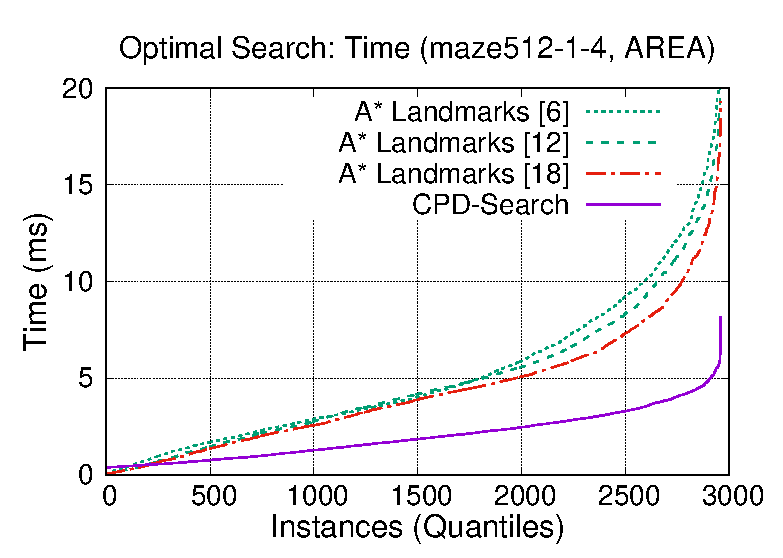
\includegraphics[width=1.0\textwidth]{src/images/optimal/maze512-1-4}
                \label{fig:optimal-maze512-1-4}
            \end{figure}
        \end{minipage}%
        \begin{minipage}{0.59\textwidth}
            \begin{figure}
                \centering
                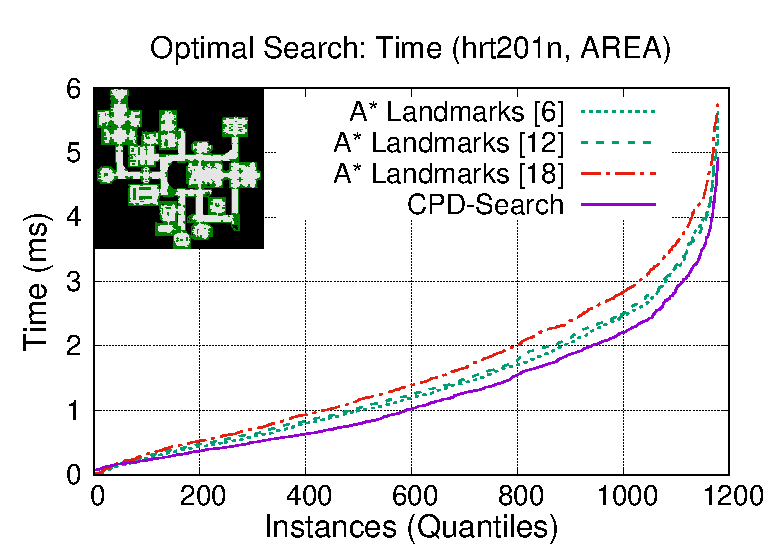
\includegraphics[width=1.0\textwidth]{src/images/optimal/hrt201n}
                \label{fig:optimal-hrt201n}
            \end{figure}
        \end{minipage}
    \end{adjustwidth}
\end{frame}

\begin{frame}{Anytime Scenario}

    In \code{hrt201n} map (almost 1200 queries):

    \begin{itemize}
        \item by 30$\mu$s \anytimeCPDSearch{} has incumbents for at least 25\% of instances, \AWA{} for almost 0\%;
        \item by 300$\mu$ \anytimeCPDSearch{} has incumbents for at least 75\% of instances, \AWA{} for at most 50\%;
        \item by 1ms \anytimeCPDSearch{} has incumbents for all instances and has computed the optimal path for at least 25\% of instances, \AWA{} has optimal paths for no instance;
        \item by 10ms \anytimeCPDSearch{} has reached the optimal solution for every instance, while \AWA{} has computed it for at most 50\%.
    \end{itemize}
\end{frame}
